% IF1014 — Apresentação (15 min cronometrados). Sem código nos slides.
% Compilação: pdflatex slides.tex (duas passadas para refs)
\documentclass[aspectratio=169]{beamer}
\usepackage[utf8]{inputenc}
\usepackage[T1]{fontenc}
\usepackage[brazil]{babel}
\usepackage{graphicx}
\usepackage{booktabs}
\usepackage{array}
\usepackage{xcolor}

\usetheme{Madrid}
\usecolortheme{seahorse}
\setbeamertemplate{navigation symbols}{}

\title[Diabetes 130-US]{Previsão de readmissão hospitalar\\\small{Diabetes 130-US Hospitals (UCI 296)}}
\subtitle{IF1014 — Mineração de Dados Aplicada (CRISP-DM)}
\author{Equipe \textit{[a preencher]}}
\institute{UFPE — 2026.1}
\date{27 de maio de 2026}

\begin{document}

\frame{\titlepage}

% ---------------------------------------------------------------
\section{Business Understanding}

\begin{frame}{Briefing do cliente}
\textbf{Cliente fictício:} SI5 Health, rede hospitalar com unidade de cuidado pós-alta.

\vspace{0.6em}
\textbf{Problema.} Identificar, na alta do paciente diabético, a probabilidade de \alert{readmissão precoce} (<30 dias) para acionar acompanhamento ativo.

\vspace{0.6em}
\textbf{Saída.} Classe $\in \{\texttt{<30}, \texttt{>30}, \texttt{NO}\}$.

\vspace{0.6em}
\textbf{Métrica de sucesso.} F1-macro no conjunto de teste (dataset desbalanceado; \texttt{<30} representa 11\%).

\vspace{0.6em}
\textbf{Restrições.} Falso negativo da classe \texttt{<30} é o erro mais caro (paciente readmite sem suporte). Limiar de operação calibrado pela capacidade do time de pós-alta.

\vspace{0.6em}
\textbf{Implicações éticas.} Viés demográfico (race, gender, age), privacidade (dados pseudonimizados), automação de decisão clínica como apoio, não substituição.
\end{frame}

% ---------------------------------------------------------------
\section{Data Understanding \& EDA}

\begin{frame}{Dataset}
Diabetes 130-US Hospitals (UCI 296, Strack et al., 2014).
\begin{itemize}
  \item 101.766 internações $\rightarrow$ 81.412 treino / 20.354 teste (split estratificado, \texttt{random\_state=42}).
  \item 47 features após remover IDs, \texttt{weight} (97\% missing), \texttt{examide}, \texttt{citoglipton}.
  \item Categóricas dominam: 24 medicações + raça, gênero, idade, diag\_1/2/3 (ICD-9 agrupado), \texttt{payer\_code}, \texttt{medical\_specialty} (alta cardinalidade).
  \item Faltantes codificados como \texttt{?} no original.
\end{itemize}
\end{frame}

\begin{frame}{EDA — pontos relevantes}
\begin{columns}
\begin{column}{0.55\textwidth}
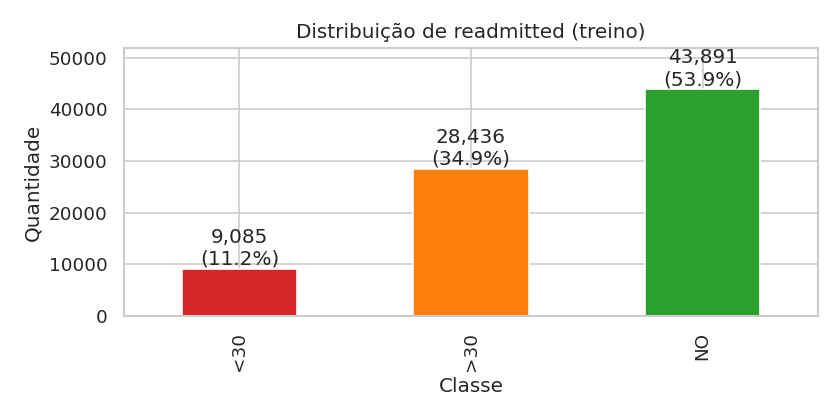
\includegraphics[width=\linewidth]{reports/figures/eda_class_balance.png}
\end{column}
\begin{column}{0.45\textwidth}
\small
\begin{itemize}
  \item Desbalanceamento: \texttt{NO} 54\%, \texttt{>30} 35\%, \texttt{<30} 11\%.
  \item \texttt{number\_inpatient}, \texttt{number\_emergency} muito assimétricas $\rightarrow$ motivam variante \textbf{RobustScaler}.
  \item Missingness pesado em \texttt{race}, \texttt{payer\_code}, \texttt{medical\_specialty}, \texttt{diag\_*}.
  \item ICD-9 com 1000+ códigos $\rightarrow$ agrupados em 9 categorias clínicas.
\end{itemize}
\end{column}
\end{columns}
\end{frame}

% ---------------------------------------------------------------
\section{Data Preparation}

\begin{frame}{Pipeline baseline}
\textbf{Limpeza estrutural} (\texttt{RawCleaner}): \texttt{?} $\rightarrow$ NaN, drop de colunas inúteis, agrupamento ICD-9, IDs como string.

\vspace{0.5em}
\textbf{ColumnTransformer}:
\begin{itemize}
  \item Numéricas: \texttt{SimpleImputer(median)} $\rightarrow$ \texttt{StandardScaler}.
  \item Categóricas: \texttt{SimpleImputer(most\_frequent)} $\rightarrow$ \texttt{OneHotEncoder(handle\_unknown="ignore")}.
\end{itemize}

\vspace{0.5em}
\textbf{Crucial:} todo \texttt{fit\_transform} acontece \alert{dentro de cada fold} da CV. Nada toca o conjunto de teste antes da Seção 9.

\vspace{0.5em}
\textbf{Variantes:} \textbf{SMOTE} (\texttt{imblearn} pipeline), \textbf{RobustScaler}, \textbf{TargetEncoder} em colunas de alta cardinalidade.
\end{frame}

% ---------------------------------------------------------------
\section{Modeling}

\begin{frame}{Os 10 algoritmos}
\centering
\begin{tabular}{ll}
\toprule
\textbf{Parte 1 (clássicos)} & \textbf{Parte 2 (avançados)} \\
\midrule
K-NN & MLP \\
LVQ (sklvq) & Comitê de MLPs (Bagging) \\
Árvore de Decisão & Stacking heterogêneo \\
SVM (\texttt{LinearSVC}) & XGBoost (GPU/CUDA) \\
Random Forest & LightGBM \\
\bottomrule
\end{tabular}

\vspace{1em}
\small
Cada modelo definido em \texttt{src/models.py} via \texttt{ModelSpec} (factory + grid + estratégia de busca: Grid ou Randomized).
\end{frame}

\begin{frame}{Busca de hiperparâmetros}
\textbf{Mesma CV em todos:} \texttt{StratifiedKFold(n\_splits=5, shuffle=True, random\_state=42)}. Comparações pareadas exigem folds idênticos.

\vspace{0.5em}
\textbf{Métrica de otimização:} \texttt{f1\_macro}.

\vspace{0.5em}
\textbf{Estratégia:} Grid em modelos com poucos HPs (DT, KNN, LVQ, Stacking); Randomized (\texttt{n\_iter=5-10}) em modelos com espaço maior (RF, LightGBM, SVM, MLP, MLP Comitê, XGBoost).

\vspace{0.5em}
\textbf{Curvas treino vs validação} salvas por configuração em \texttt{reports/figures/<modelo>\_\_<tag>\_\_train\_vs\_val.png} (uma figura por modelo $\times$ pré-processamento).
\end{frame}

% ---------------------------------------------------------------
\section{Evaluation}

\begin{frame}{Baseline — F1-macro por modelo}
\centering
\small
\begin{tabular}{lccc}
\toprule
\textbf{Modelo} & \textbf{F1-macro CV} & \textbf{$\sigma$ folds} & \textbf{Gap treino-val} \\
\midrule
Random Forest        & \textbf{0.4512} & 0.0028 & 0.39 \\
SVM (LinearSVC)      & 0.4471 & 0.0024 & 0.01 \\
XGBoost (GPU)        & 0.4240 & 0.0023 & 0.21 \\
LightGBM             & 0.4204 & 0.0017 & 0.28 \\
Stacking             & 0.4167 & 0.0021 & 0.06 \\
MLP                  & 0.4121 & 0.0115 & 0.02 \\
Decision Tree        & 0.4012 & 0.0013 & 0.28 \\
K-NN                 & 0.3951 & 0.0021 & 0.19 \\
LVQ (GLVQ)           & 0.2648 & 0.0024 & 0.00 \\
\textit{Comitê MLPs}* & \textit{em execução} & --- & --- \\
\bottomrule
\end{tabular}

\vspace{0.3em}
\footnotesize $^*$resultado a inserir após término da busca.

\vspace{0.5em}
\textbf{Observação.} RF e SVM lideram porque a busca selecionou \texttt{class\_weight="balanced"} (já endereça desbalanceamento na fase de Modeling). LVQ é o mais fraco — protótipos sofrem em 200+ features OHE.
\end{frame}

\begin{frame}{Comparação baseline vs variantes (parcial)}
\textbf{Critério de promoção:} diferença positiva \emph{e} p<0.05 em Wilcoxon ou paired t-test (5 folds pareados).

\vspace{0.5em}
\centering
\footnotesize
\begin{tabular}{llrrcc}
\toprule
\textbf{Modelo} & \textbf{Variante} & $F1_{\text{base}}$ & $F1_{\text{var}}$ & $\Delta$ & p (paired t) \\
\midrule
Decision Tree & SMOTE        & 0.4012 & 0.4190 & \textbf{+0.0178} & \textbf{0.007}$^{*}$ \\
Decision Tree & RobustScaler & 0.4012 & 0.4012 & +0.0000 & 0.933 \\
Decision Tree & TargetEnc    & 0.4012 & 0.4067 & \textbf{+0.0055} & \textbf{0.042}$^{*}$ \\
LVQ           & SMOTE        & 0.2648 & 0.3921 & \textbf{+0.1273} & \textbf{$<$0.001}$^{*}$ \\
LVQ           & RobustScaler & 0.2648 & 0.2719 & \textbf{+0.0071} & \textbf{0.003}$^{*}$ \\
LVQ           & TargetEnc    & 0.2648 & 0.2721 & \textbf{+0.0072} & \textbf{$<$0.001}$^{*}$ \\
Stacking      & RobustScaler & 0.4167 & 0.4164 & --0.0004 & 0.474 \\
Stacking      & TargetEnc    & 0.4167 & 0.4145 & --0.0022 & 0.062 \\
KNN           & TargetEnc    & 0.3951 & 0.3854 & --0.0097 & --- \\
\bottomrule
\end{tabular}

\vspace{0.3em}
\footnotesize $^{*}$ = p<0.05. \emph{Wilcoxon} mais conservador (5 folds só dão p=0.0625 mesmo com sinal consistente).

\vspace{0.5em}
\textbf{Leitura.} SMOTE \alert{ajuda} DT e LVQ (modelos sem balanceamento embutido). Não foi rodado em modelos que já tinham \texttt{class\_weight="balanced"} (RF, SVM).

\vspace{0.3em}
\textit{Outros pares (LGBM, XGB, RF, MLP × 3 variantes) ainda executando.}
\end{frame}

\begin{frame}{Modelo vencedor (parcial)}
\textbf{Líder atual:} \alert{Random Forest baseline} — F1-macro = \textbf{0.4512 $\pm$ 0.0028}.

\vspace{0.6em}
\textbf{Hiperparâmetros vencedores:}
\begin{itemize}
  \item \texttt{n\_estimators=200}, \texttt{max\_depth=20}, \texttt{max\_features="log2"}
  \item \texttt{min\_samples\_leaf=1}, \alert{\texttt{class\_weight="balanced"}}
\end{itemize}

\vspace{0.4em}
\textbf{Por quê esse vence:}
\begin{itemize}
  \item Maior F1-macro entre todas as combinações já avaliadas.
  \item Diferença vs 2º colocado (SVM) é \emph{não significativa} (Wilcoxon p=0.125): ambos sustentam o pódio.
  \item \texttt{class\_weight="balanced"} ataca o desbalanceamento sem custo de SMOTE.
  \item Curva treino vs val mostra overfit moderado ($F1_{tr}=0.84$, $F1_{val}=0.45$) — mas estável entre folds ($\sigma=0.003$).
  \item Inferência rápida (~ms por amostra), interpretabilidade via importância de features.
\end{itemize}

\vspace{0.4em}
\footnotesize \textit{Ranking pode mudar quando variantes de LGBM/XGB/MLP terminarem (estimativa: 30-60min).}
\end{frame}

\begin{frame}{Avaliação final no teste}
\textit{(Preencher após executar a Seção 9.)}

\begin{columns}
\begin{column}{0.45\textwidth}
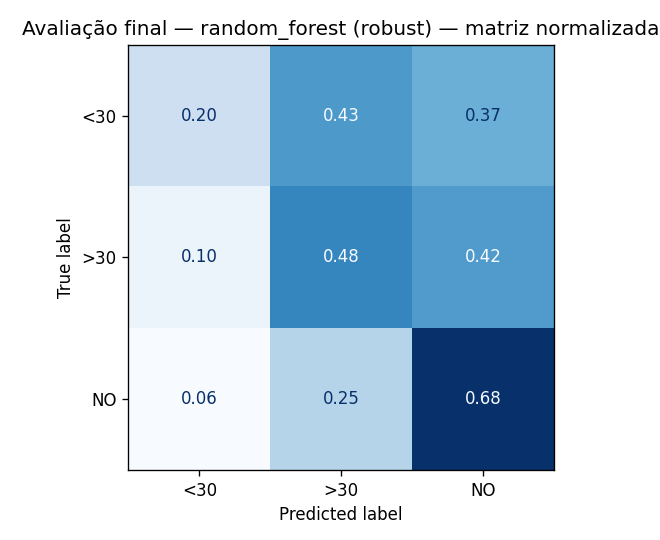
\includegraphics[width=\linewidth]{reports/figures/final_confusion.png}
\end{column}
\begin{column}{0.55\textwidth}
\small
\textbf{F1-macro teste:} \emph{X.XXXX}\\
\textbf{F1-macro CV:} \emph{X.XXXX ± X.XXXX}\\
\textbf{$\Delta$ teste $-$ CV:} \emph{$\pm$X.XXXX}\\
\textbf{Balanced accuracy:} \emph{X.XXXX}\\
\textbf{ROC-AUC macro:} \emph{X.XXXX}\\
\textbf{PR-AUC macro:} \emph{X.XXXX}

\vspace{0.5em}
\textbf{recall(\texttt{<30}):} \emph{X.XXX}\\
\emph{(métrica operacional crítica)}
\end{column}
\end{columns}
\end{frame}

% ---------------------------------------------------------------
\section{Deployment}

\begin{frame}{Deployment e riscos}
\textbf{Uso.} Score acionado na alta; pacientes \texttt{<30} entram em fila de acompanhamento (ligação 48h, retorno 7d, revisão farmacoterapia).

\vspace{0.5em}
\textbf{Calibração.} Threshold tuning sobre \texttt{predict\_proba(<30)} para maximizar recall sujeito ao teto de fila operacional.

\vspace{0.5em}
\textbf{Riscos:}
\begin{itemize}
  \item Viés demográfico (race/age/gender). Mitigação: auditoria DIR por subgrupo, F1-macro estratificado mensal.
  \item Drift de população (nova unidade, mudança de mix). Mitigação: PSI semanal nas top-15 features.
  \item Privacidade: pseudonimização, sem retenção de raw fora de \texttt{data/raw/}.
\end{itemize}

\vspace{0.5em}
\textbf{Retreinamento.} Gatilhos: PSI>0.25 em $\geq$3 features, F1 mensal cai >0.05 vs teste, ou trimestralmente.
\end{frame}

% ---------------------------------------------------------------
\section{Encerramento}

\begin{frame}{Reprodutibilidade}
\textbf{1 comando de setup, 1 de execução.}

\vspace{0.3em}
\small
\texttt{uv sync}\\
\texttt{uv run jupyter nbconvert --to notebook --execute main.ipynb}

\vspace{0.6em}
\textbf{Artefatos versionados:} \texttt{reports/cv\_results/*.csv} (cv\_results\_ completo por modelo $\times$ variante), \texttt{reports/figures/*.png} (curvas treino vs val, matriz, ROC, PR, barras).

\vspace{0.5em}
\textbf{Integridade do split:} \texttt{load\_test} levanta \texttt{PermissionError} sem o token \texttt{I\_AM\_IN\_FINAL\_EVALUATION}. Token aparece apenas na Seção 9 do notebook.

\vspace{0.5em}
\textbf{Uso de IA generativa.} Declarado (Seção 14 das exigências): Claude Opus 4.7 usado para apoio em codificação, revisão e documentação. Decisões metodológicas (split, métrica, escolha de modelos e variantes, leitura dos resultados) conduzidas pela equipe.
\end{frame}

\begin{frame}{Obrigado}
\centering
\Large Perguntas?

\vspace{1em}
\small
Repositório: \emph{[link privado, professor adicionado]}

\vspace{0.5em}
Equipe: \emph{[nomes]}
\end{frame}

\end{document}
